%*----------- SLIDE -------------------------------------------------------------
\begin{frame}[t]{Cronogram} 
    The project had the start in\textbf{02/11/2022} and has its end aimed to \textbf{04/01/2022}.
    %\newline
    \begin{center}
        %\centerline{
            \begin{figure}
                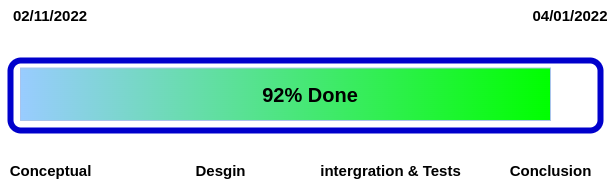
\includegraphics[width=.9\textwidth]{92.png}
            \end{figure}
        %}
    \end{center}

       
\end{frame}
%-


\begin{frame}[t]{Introduction} 
    \transdissolve[duration=0.5]
    The \textbf{manipulators are autonomous} tools that have a lot of functions. Their use is increasing a lot  and in \textbf{many fields}.
    The \textbf{Jax Manipulator} challenge has a goal to use the \textbf{JeRo Timon} to an autonomous  task.  


    \begin{center}
        %\centerline{
            \begin{figure}
                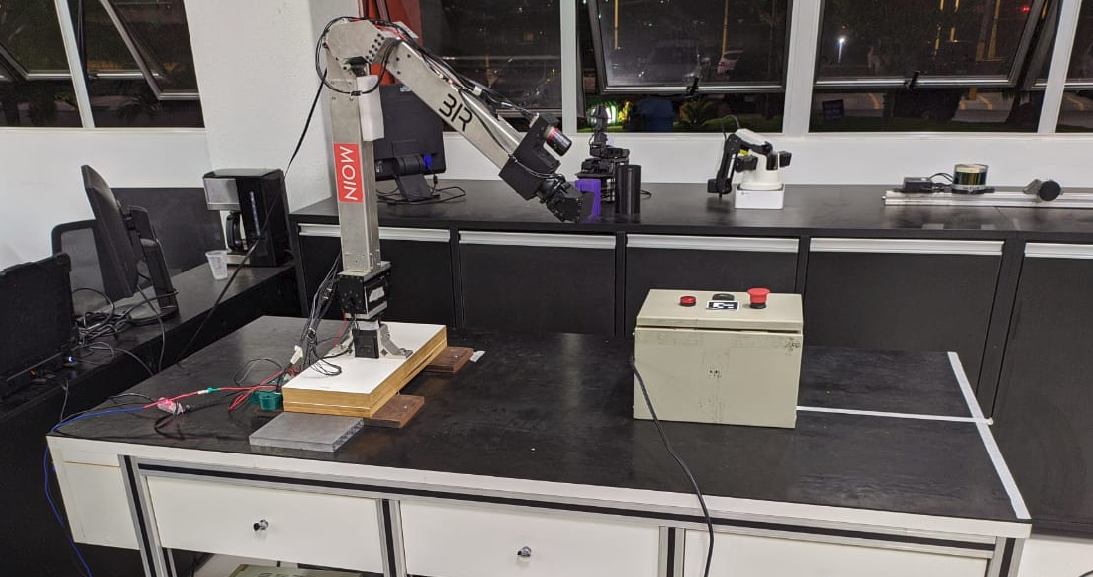
\includegraphics[width=.65\textwidth]{TIMAO.png}
            \end{figure}
        %}
    \end{center}
    %\newline
       
\end{frame}
%-

\begin{frame}[c]{The Task}

    The tasks require that Jero Timon manipulators \textbf{find a tag that}  is placed in a specific position.
    after the tag is found, the manipulator should \textbf{push a button} that is located at an box.

    \begin{center}
        %\centerline{
            \begin{figure}
                
\includegraphics[width=.9\textwidth]{task.png}
            \end{figure}
        %}
    \end{center}

\end{frame}



\begin{frame}[c]{Functionalities}

    The robot is able to identify the tag with applications of  computer vision tools. The moves in the space are acquired by the trajectory control that uses both forward kinematics and inverse kinematics.

    \begin{center}
        %\centerline{
            \begin{figure}
                
\includegraphics[width=.9\textwidth]{functions.png}
            \end{figure}
        %}
    \end{center}


\end{frame}





\begin{frame}[c]{Intergration}

    

    \begin{center}
        %\centerline{
            \begin{figure}
                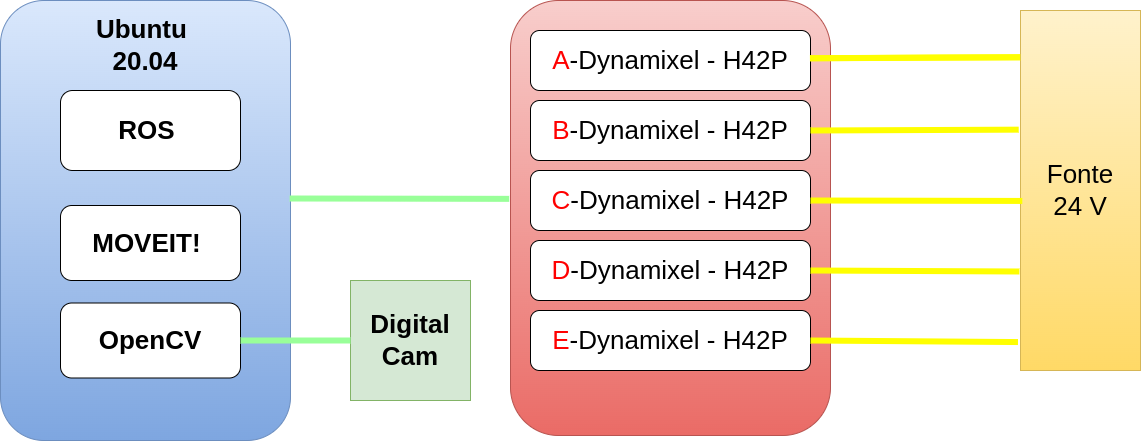
\includegraphics[width=.9\textwidth]{intergration.png}
            \end{figure}
        %}
    \end{center}


\end{frame}


\begin{frame}[c]{System}

    

    \begin{center}
        %\centerline{
            \begin{figure}
                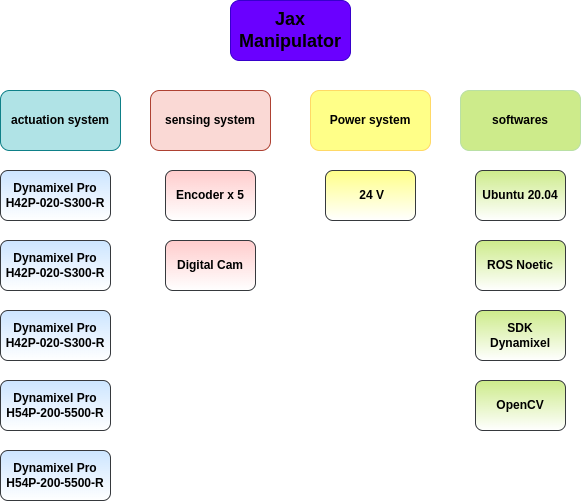
\includegraphics[width=.55\textwidth]{jax_systems.png}
            \end{figure}
        %}
    \end{center}


\end{frame}




\begin{frame}[c]{Tests}

    Many Tests were performed to verify the functionality of the manipulator. Some tests were:

    \begin{enumerate}
        \item Verify  the URDF of the robot;
        \item Verify  the behaivor of the joints;
        \item observe the movement of the manipulator;
        \item Observe how the forward  and inverse kinematics perform.
        \item Detect the tag in the enviorment.
        \item Visualze the state of robot.
    \end{enumerate}

  


\end{frame}



\begin{frame}[c]{State Machine}

   To perform the challenge, the robot must follow a state machine.

     \begin{center}
        %\centerline{
            \begin{figure}
                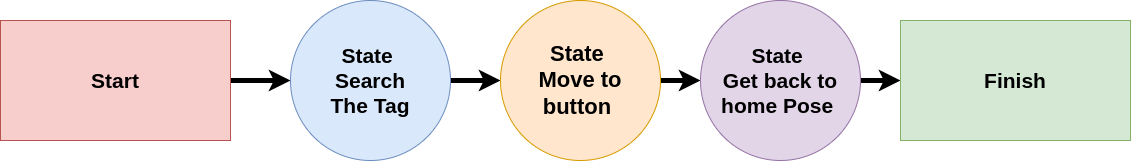
\includegraphics[width=.90\textwidth]{STATE.png}
            \end{figure}
        %}
    \end{center}


\end{frame}



\begin{frame}[c]{Demostration}

    \begin{figure}
        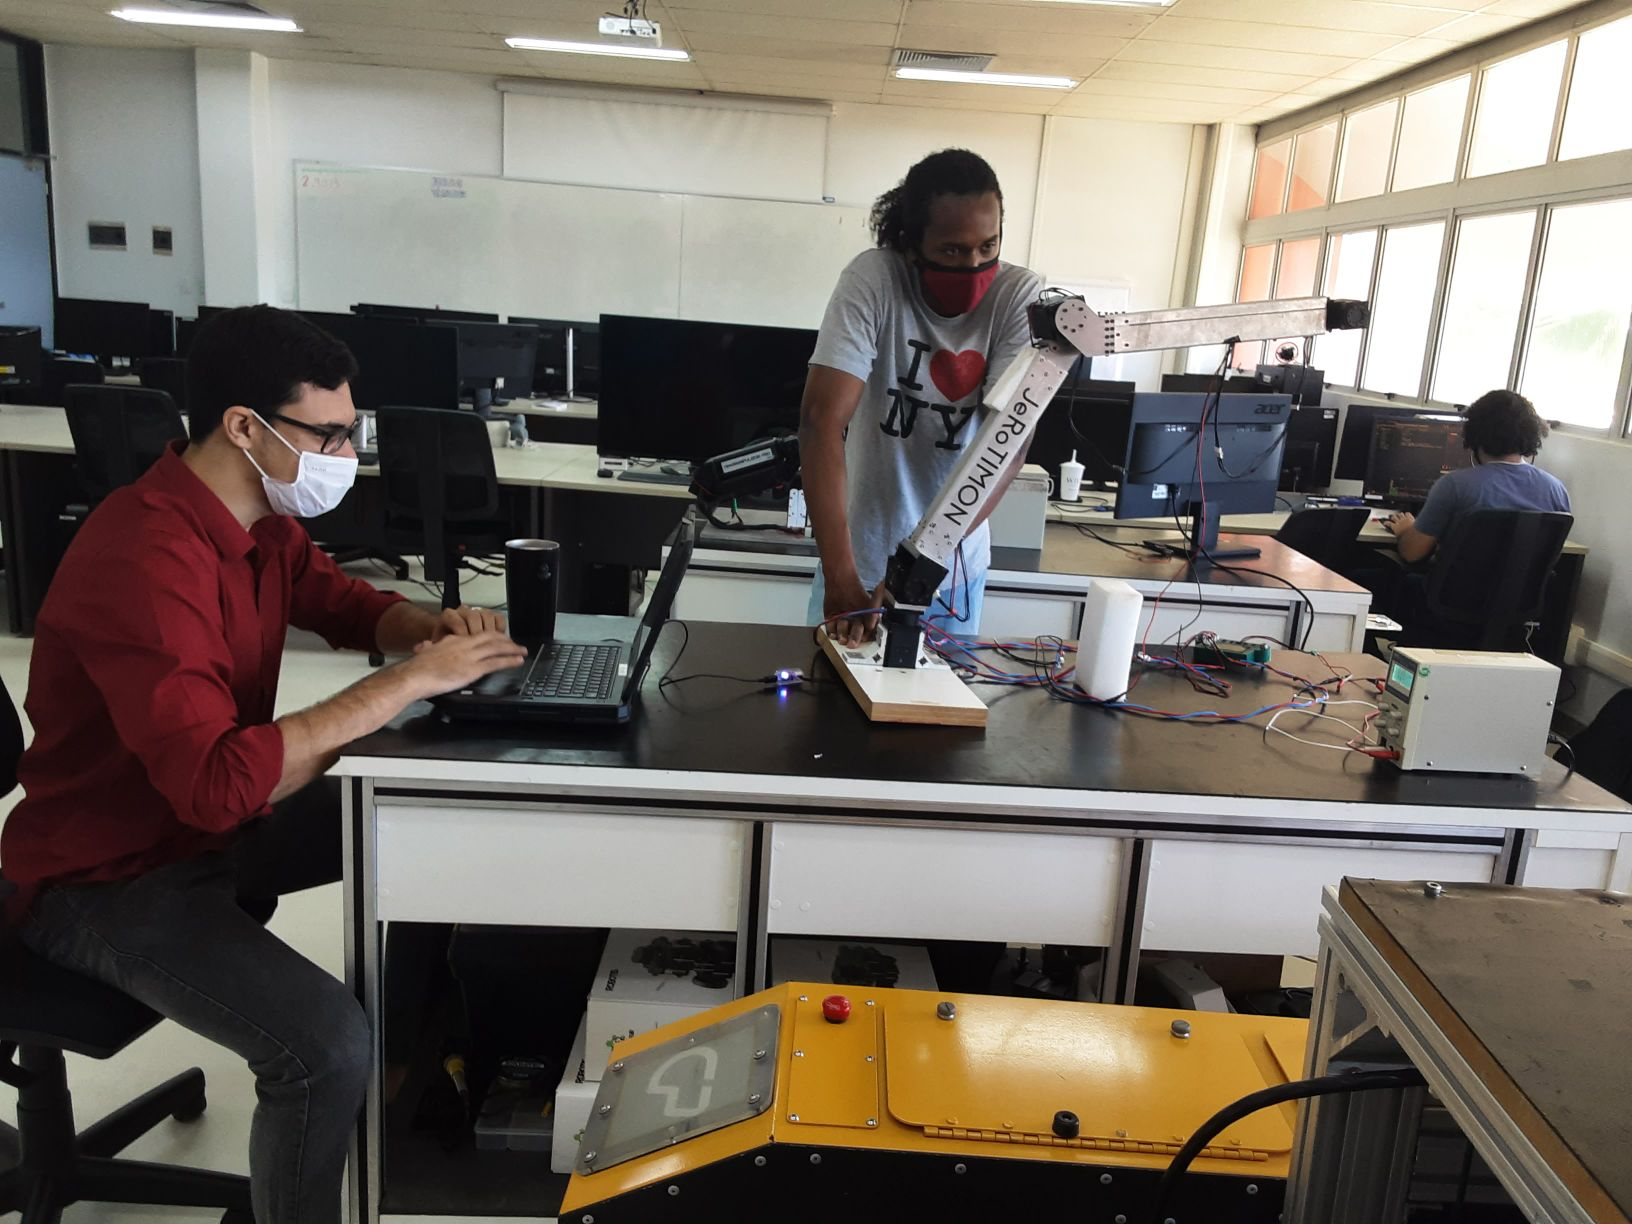
\includegraphics[width=.60\textwidth]{demo.jpg}
    \end{figure}
 
 \end{frame}
%*----------- SLIDE -------------------------------------------------------------
%\begin{frame}[c]{Objetivo} 
%    \framesubtitle{sub-objetivo}
%    \transdissolve[duration=0.5]
%   
%    \begin{center}
%        \Wider{%
%        \begin{shaded}
%        \begin{center}
%            \vspace*{0.5cm}
%            \resizebox{!}{0.7cm}{%
%                \color{bg} O objetivo é ter um objetivo.
%            }%
%        \end{center}
%        \end{shaded}
%        }%
%    \end{center}
%    
%   
%%*----------- notes
%    \note[item]{Notes can help you to remember important information. Turn on the notes option.}
%\end{frame}
%-


%-
